\documentclass[a4paper,12pt]{article}
\usepackage[utf8]{inputenc}
\usepackage[T1]{fontenc}
\usepackage[english]{babel}
\usepackage[nottoc]{tocbibind}
\usepackage{graphicx}
\usepackage{geometry}
\geometry{a4paper,
		     tmargin = 35mm, 
		     lmargin = 30mm,
		     rmargin = 30mm,
		     bmargin = 30mm}
\usepackage{mathtools}
\usepackage{amsmath}
\usepackage{color}
\usepackage{setspace}
\usepackage{amsmath,amssymb}
\usepackage{float}

\usepackage{indentfirst}

\usepackage{listings}
\usepackage{afterpage}
\usepackage[font=small,labelfont=bf]{caption}
\pagestyle{plain}

\definecolor{dkgreen}{rgb}{0,0.6,0}
\definecolor{gray}{rgb}{0.5,0.5,0.5}
\definecolor{mauve}{rgb}{0.58,0,0.82}

\lstset{frame=tb,
language=Python,
aboveskip=4mm,
belowskip=4mm,
showstringspaces=false,
columns=flexible,
numbers=none,
keywordstyle=\color{blue},
numberstyle=\tiny\color{gray},
commentstyle=\color{dkgreen},
stringstyle=\color{mauve},
breaklines=true,
breakatwhitespace=true,
tabsize=3
}

\usepackage[hidelinks]{hyperref}

\hypersetup{
  colorlinks   = true, %Colours links instead of ugly boxes
  urlcolor     = blue, %Colour for external hyperlinks
  linkcolor    = blue, %Colour of internal links
  citecolor   = green  %Colour of citations
}

\renewcommand{\thesection}{\Roman{section}.}
\renewcommand{\thesubsection}{\Roman{section}. \arabic{subsection}.}
\renewcommand{\thesubsubsection}{\Roman{section}. \arabic{subsection}.\arabic{subsection}.}

\begin{document}

\linespread{1.2}

\begin{titlepage}

	\centering
	
\includegraphics[width=0.66\textwidth]{elte.jpg}\par\vspace{1cm}
	{\scshape\LARGE Eötvös Loránd University \par}
	\vspace{1cm}
    \rule{140mm}{0.1mm}\\
    \vspace{.5cm}
	{\scshape\Large Scientific imaging \\ using artificial neural networks \\ in medicine\par}
	\vspace{.5cm}
	\rule{140mm}{0.1mm}\\
	\vspace{.5cm}
	{\large\itshape Olar Alex\par}
	\vfill
	supervisor\par
	\vspace{0.5cm}
	{\Large Prof. István Csabai}

	\vfill
	
	{\large 2020 \par}
\end{titlepage}

\begin{abstract}

In 2012 a neural network based architecture won the ImageNet Large Scale Visual Recognition Challenge (ILSVRC) \cite{russakovsky2015imagenet} in object classification. The model was called AlexNet \cite{krizhevsky2012imagenet} named after the creator Alex Krizhevsky. In 2015 a new network from Microsoft Research called ResNet \cite{he2016deep} surpassed human performance in the classification task of ILSVRC and won the Common Objects in Context (COCO) \cite{lin2014microsoft} detection challenge as well. Object localization, segmentation and image classification since then improved vastly and is still improving to this day. New techniques and state-of-the-arts come out on a daily basis and it is extremely difficult to keep up with the surge of scientific papers in computer vision and related fields. This has not remained without attention in biology nor medicine. Computer aided diagnostics systems has been deployed long before deep learning prevailed but they were ignored or rarely used. As of now, scientists at Google just announced that they have surpassed radiologists in reading mammography images for breast cancer screening \cite{mckinney2020international}, there are ongoing challenges and research for prostate cancer screening as well as stomach cancer screening \cite{li2019signet}. All of these techniques apply some newly emerged computer vision algorithms to enable clinical workers and doctors to work more efficiently and of course to lighten the burden that comes with national screening programs and countless work hours and to advance microscopes as well \cite{chen2019augmented}. In this work I present results and methods regarding computer aided diagnostics in colorectal cancer screening that was done collaboratively with Semmelweis University as well as techniques from a project applied to detect glial cells in human brain tissue in collaboration with Semmelweis University and automatic scoring of X-ray images for rheumatoid arthritis (RA2) patients in a Dream Challenge \cite{bionetworks}.

\end{abstract}

\newpage

\tableofcontents

\newpage

\section{Introduction}

\vspace{7mm}

\subsection{General}

\vspace{7mm}

Neural networks are universal function approximators that are organized into layers. Layers of a neural network can be highly specialized, such as convolutional layers, that can efficiently learn spatial features, others might simply do matrix multiplication and apply a non-linear mapping to the input in order to extract underlying information from the data. A neural network architecture nowadays is a concatenation of differentiable layers and training means adjusting the tunable weights of these layers simultaneously based on input data and an objective/loss function that we aim to minimize.

\vspace{4mm}

\par Computer vision for many years was based on hand-engineered feature extraction and although convolutional neural networks (CNNs) were used for some dimensionally constrained problems, such as hand-written digit recognition \cite{lecun1998gradient}. The breakthrough for CNNs came with the advent of graphical processing units (GPUs). As these processors have become widely available due to computer gaming the hardware wass pushed to its limits and manufacturers poured a lot of money into research. Therefore the GPUs not only did include more and more on-board memory year-by-year but also performance was improving rapidly. Since computer graphics requires a lot of matrix multiplication and concurrent, parrarellized computation the scientific community jumped on it and started using graphical processors.

\vspace{4mm}

\par The ImageNet Large Scale Visual Recognition Challenge \cite{ILSVRC15} was launced in 2010 with approximately 1.2 million images containing 1000 categories. The goal of the challenge was to classify images into these categories on a held out test set that was not provided for the participants beforehand. In 2011 a 25\% top-5 error rate was already considered very good but in 2012 the first convolutional neural network based model \cite{krizhevsky2012imagenet} won the challenge beating the top results by a huge margin. In order to do so good they used GPUs heavily and proved that image classification is possible via CNNs on large scale images as well.

\vspace{4mm}

\par Soon after the re-discovery of convolutional networks for image recognition tasks the scientific community in computer vision realized that convolutional neural networks learn generalizable features and the datasets they considered different so far are not so distinct after all. Networks trained on a dataset of recognizing 1000 different classes can be transferred to other datasets with the change of the top of the network to recognize fundamentally different images. This method is called tranfer learning and is exceedingly used nowadays thanks to its efficiency.

\vspace{4mm}

\par Soon enough human performance was surpassed \cite{he2016deep} by the ResNet architecture and since then people are arguing whether there is still need on improving ImageNet performance because it is soo good. In response to that the ILSVRC stopped in 2017 to focus on other problemsets. 

\vspace{7mm}

\subsection{Motivation}

\vspace{7mm}

Currently deep learning is everywhere and almost everyone is trying to use it in order to achieve better accuracy in some task. In the industry the main application for artificial intelligence (AI) is to develop self-driving cars in addition to improve recommendation systems for online commercials. On the other hand, it would be highly beneficial for modern societies to use computer vision for better healtcare, education, road safety.

\vspace{4mm}

\par Google has partnered with the United Kingdom's health system ( NHS - National Health System ) to gather all the data they can to improve diagnostics and to build algorithms that can work for medics and sanitary workers in order to improve healthcare. This all sounds to good to be true in capitalism and it is. This has caused outrage amongst the people of the UK \cite{kollewe_2019} but they have some undeniable results regarding reading mammograms better then radiologists \cite{mckinney2020international}. We are in an era where governments can lead large-scale projects (in data size) in order to improve their healthcare systems without investing vast amounts of money for equipment. The COVID-19 crisis showed that with enough data and computational resources pneumonia detection can be achieved with high accuracy \cite{nvidia}.

\vspace{4mm}

\par In my opinion computer vision has achieved a state that almost every vision related task can be done on human performace level or even surpassed by computers. Such as glial cell detection in mouse brain tissue \cite{suleymanova2018deep}, reading mammograms  \cite{ribli2018detecting}, 
predicting colorectal cancer outcome \cite{skrede2020deep}, volumetric data such as CTs \cite{cciccek20163d}. I could also mention advancement in weak-lensing, astrophysics \cite{ribli2019improved} and new areas to explore, such as Hamiltonian \cite{greydanus2019hamiltonian} and Largrangian \cite{cranmer2020lagrangian} neural networks for physics. It is also worth to mention advancement in reinforcement learning that started with playing Atari games \cite{mnih2013playing} successfully and on-par with human players and led to playing Dota 2 and Starcraft \cite{alphastarblog} in top-tier leagues. This might sound irrelevant but reinforcement learning robots will take over jobs of production line workers \cite{satariano_metz_2020} in the very near future.

\vspace{4mm}

\par Therefore it is the right time to do research in the widespread application of AI in the medical field and I am certain that doing something here is highly beneficial not only for career self-advencement but also for the society as well. 

\vspace{7mm}

\subsection{Overview}

\vspace{7mm}

//TODO: sum up everything here that comes

\newpage

\section{Computer vision}

\vspace{7mm}

\subsection{Vision}

\vspace{7mm}

\par The human visual cortex is composed of many hierarchical layers but the image data required by our eyes is processed through cells on the retina that are sensitive to light known as the rods and cones. The rods are sensitive to colour whilst the cones are sensitive for intensitiy of the photons. The number of cones is significantly higher then the number of rods, therefore we are much more adapted to detecting light intensity than to colours. The are three types of these cone cells causing trichromacy \cite{arrese2002trichromacy} and therefore in computer science the most widespread format of images is stored in RGB (red-green-blue) channels. The visual cortex is basically doing edge detection in the V1 (primary visual cortex) which has been computationally reproduced \cite{olshausen1996emergence} while it is assumed that the V2 \cite{ZiembaV2} and V4 are doing much more abstract representations, the latter already producing objects.

\vspace{7mm}

\subsection{Convolutional neural networks}

\vspace{7mm}

\par All these arguments inspired many layered convolutional neural networks that are doing computations spatial data such as images. Convolutions are about learning sliding kernels on three dimensional image data (two spatial dimensions and color channels, 2 + 1) these kernels provide efficient and translation invariant parameters for the models. The convolutional operation is relatively simple and straight-forward. On one dimensional sequences and functions it is defined as:

\begin{align*}
    (u * v)_n = \sum_{m = -\infty}^{\infty} u_{m} v_{n-m} \\
    (f * g)(t) = \int_{-\infty}^{\infty} f(\tau)g(t-\tau)d\tau
\end{align*}

\vspace{4mm}

\par Spatially this is defined similarly but for a finite $K$ kernel with size $(k_1, k_2)$:

\vspace{4mm}

\begin{align*}
    (I * K)_{ik} = \sum_{m = 1}^{k_1}\sum_{n = 1}^{k_2} I_{i - m, k - n} K_{m, n}
\end{align*}

\vspace{4mm}

\par This can be visually illustarted by the figure below where the parameters of $K$ on the image is learned algorithmically by seeing lots of examples:

\vspace{4mm}

\begin{figure}[H]
    \centering
    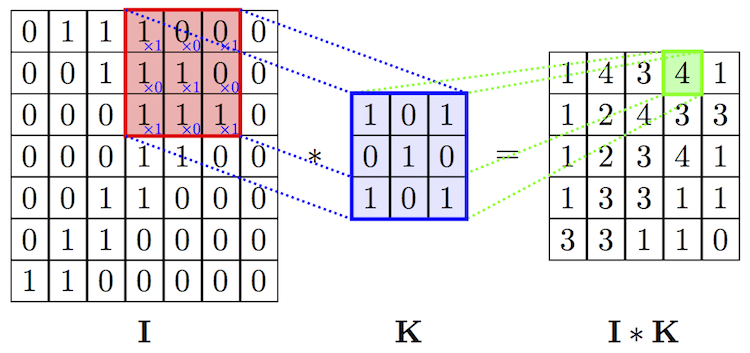
\includegraphics[width=0.7\linewidth]{An-example-of-convolution-operation-in-2D-2.png}
    \caption{2D convolution - Scientific Figure on ResearchGate. Available from: \url{https://www.researchgate.net/figure/An-example-of-convolution-operation-in-2D-2_fig3_324165524} [accessed 31 Mar, 2020]}
    \label{fig:2d-conv}
\end{figure}

\vspace{4mm}

\par There are two main branches of machine learning, such as suprvised and unsupervised learning. In applications of computer vision supervised learning is used most of the time. These are methods for image classification, object detection/segmentation. These all work by defining an objective function we want to minimize in order to achieve a desired rate of error. 

\subsubsection{Binary classification}

\par The simplest case is probably binary classification. In binary classification we want to maximize the joint probability of getting a data point $x$ and by applying a function $f(x, \theta) = \hat{y}$, where $\theta$ are function parameters, we predict $\hat{y}$ probability for $x$ being in class $1$ and therefore $1 - \hat{y}$ probability for being in class $0$. If $y$ is the true label of the data point, then we can formalize our explanation as:

\vspace{4mm}

\begin{align}
    P(y = 1 | x) = \hat{y} \\
    P(y = 0 | x) = 1 - \hat{y} \\
    \quad \rightarrow P(y | x) = \hat{y}^{y} \cdot (1 - \hat{y})^{(1-y)}
\end{align}

\vspace{4mm}

\par We want to maximize the sum of this joint probability for all the examples we have in a dataset but we can do so by taking the logarithm of this since the logarithm function is bijective. We call this our objective or loss function we aim to minimize:

\vspace{4mm}

\begin{equation}
    L\big(y, \hat{y}\big) = -\sum_{i = 1}^{N_{data}} \Big(y^{(i)}\log\hat{y}^{(i)} + (1 - y^{(i)})\log(1 - \hat{y}^{(i)})\Big)
\end{equation}

\vspace{4mm}

\par As we acquired $\hat{y}^{(i)}$ by a function $f(x^{(i)}, \theta) = \hat{y}^{(i)}$ on the data point $x$ with parameters $\theta$ therefore the objective function is parametrized by $\theta$ as well. So by feeding examplary data points to $f$ and calculating the loss we could also calculate the corresponding derivatives of the loss to the parameters $\frac{\partial L}{\partial \theta}$ and apply these derivatives with a pre-defined rate $\mu$ in order to improve the objective. We call this gradient descent since the gradient of the function gives the biggest slope on the multidimensional surface spanned by $\theta$ and if we move to the oppositve direction of the gradients we then minimize the diseired function. We call it batch stochastic gradient descent (SGD) if only a batch of samples is used due to computational resource limitations. This intoruduces noise to the learning process but if we sample the data uniformly we could still improve the objective function in many iterations:

\vspace{4mm}

\begin{equation}
    L_{batch} = - \sum_{\#batch\_size}L(y^{(i)}, \hat{y}^{(i)}) = L_{batch}(\theta)  
\end{equation}

\vspace{4mm}

\par The gradient with respect to (w.r.t) $\theta$ can be applied with batch SGD in the update step after each sample of data points:

\vspace{4mm}

\begin{equation}
    \theta = \theta - \mu \frac{\partial L}{\partial \theta}
\end{equation}

\vspace{4mm}

\par As it is evident from above any type of differentiable objective function can be used with any differentiable model $f$ and the model can be trained on samples of dataset in order to yield a successful predictor for previously unseen datapoints. The aim of computer vision is to be able to generalize algorithms as much as possible. The success of deep learning and convolutional neural networks lies in generalization since with large enough datasets they have very close performance on unseen data as on training data. Therefore we could train a model to recognize lung damage on CT scans on a large enough dataset and apply it in every hospital in the world where they have a gaming graphics card. This solution is pheasible and can improve healthcare tremendously. For lower-risk applications it is even possible to run models in the browser using WebGL technology that recognizies the graphics capabilities of the underlying machine and uses it in order to run trained models \cite{cohen2019chester}.

\newpage

\bibliographystyle{unsrt}
\bibliography{references}

\end{document}\grid
